\section{光滑目标的最优条件}
\label{sec:opt-prob-optimality}

前两节的条件是几何的：可行域是否紧、目标是否凸。要真正判断某个候选是不是最优，我们需要能在这一点上计算的条件。目标可微时，多元微积分把函数在一点附近写成梯度项、Hessian二次型与高阶余项之和，这些局部量就成了判别工具。本节只处理可行域内部的点，等价于在该点附近做无约束比较；边界上的最优条件需要可行方向与乘子，留给第~\ref{chap:constrained-optimization}章。卷一已经从多元函数的角度建立了极值的一阶、二阶条件（可参考\BookChapterRef{chap:multivariate-calculus}{卷一“多元函数微分”章}），这里从优化的角度重新组织它们：哪些是必要条件，哪些是充分条件，什么时候局部判据能推出全局结论。

\subsection{一阶条件与驻点}
\label{sec:opt-prob-first-order}

\paragraph{沿每个方向看}
站在最低点上，朝任何方向迈一小步都不会更低。把这句话变成计算：固定方向$\bm d$，只看沿直线$\bm x^\star+t\bm d$的一元函数$\phi(t)=f(\bm x^\star+t\bm d)$。若$\bm x^\star$是局部最优解且在可行域内部，$\phi$在$t=0$处有局部最小，它的导数$\phi'(0)=\langle\nabla f(\bm x^\star),\bm d\rangle$不能为负；对$-\bm d$同样如此，于是它只能为零。

\begin{theorem}[一阶必要条件]
\label{thm:opt-prob-first-order-necessary}
设$\bm x^\star$是$C$的内点，即存在$r>0$使$B(\bm x^\star,r)\subseteq C$；$f$在$\bm x^\star$处可微。若$\bm x^\star$是$f$在$C$上的局部最优解，则$\nabla f(\bm x^\star)=\bm 0$。
\end{theorem}

\begin{proof}
对任意$\bm d$，$|t|$充分小时$\bm x^\star+t\bm d\in C\cap B(\bm x^\star,r')$，其中$r'$是局部最优的邻域半径。于是$\phi(t)=f(\bm x^\star+t\bm d)\geq\phi(0)$。当$t>0$时，$(\phi(t)-\phi(0))/t\geq0$，令$t\downarrow0$得$\langle\nabla f(\bm x^\star),\bm d\rangle\geq0$。以$-\bm d$代替$\bm d$得相反不等式，所以$\langle\nabla f(\bm x^\star),\bm d\rangle=0$对所有$\bm d$成立，取$\bm d=\nabla f(\bm x^\star)$即得梯度为零。
\end{proof}

梯度为零的点称为\term{驻点}（stationary point）。一阶条件只是必要条件，它的局限有三方面。第一，驻点不一定是最小点：$-\lVert\bm x\rVert_2^2$在原点有驻点，那里是最大点；$x^2-y^2$在原点也有驻点，沿$x$轴是最低点、沿$y$轴是最高点，这样的驻点称为\term{鞍点}（saddle point）。第二，定理只对内点成立：示例~\ref{ex:opt-prob-local-global}中，$C=[-1.5,1.5]$上的全局最优解$x=1.5$在边界上，导数是$-1.875$而不是零。第三，即使驻点是局部最优，也不一定是全局最优：同一函数在$x=-1$处导数为零且是局部最优，却比$C$上的最优值高得多。

\paragraph{凸目标的驻点是全局最优}
凸性把这个必要条件变成充分条件。若$f$在开凸集$D$上凸且可微，$\nabla f(\bm x^\star)=\bm 0$，代入一阶支撑下界~\eqref{eq:opt-prob-first-order-support}，对任意$\bm v\in D$，
\[
  f(\bm v)\geq f(\bm x^\star)+\langle\bm 0,\bm v-\bm x^\star\rangle=f(\bm x^\star).
\]

\begin{theorem}[凸目标驻点的全局最优性]
\label{thm:opt-prob-convex-stationary}
设$D$是开凸集，$f:D\to\mathbb R$凸且可微。则$\bm x^\star\in D$是$f$在$D$上的全局最优解，当且仅当$\nabla f(\bm x^\star)=\bm 0$。
\end{theorem}

必要性来自定理~\ref{thm:opt-prob-first-order-necessary}（开集中每点都是内点），充分性就是上面的一行计算。几何上，切平面是全局下界，水平的切平面就把最小值钉在了切点上。

这个结论的价值在于：对凸目标，求解优化问题等价于解方程$\nabla f=\bm 0$，并且找到的任何一个解都是全局最优。最小二乘的梯度为$\nabla f(\bm x)=\bm A^\top(\bm A\bm x-\bm b)+\lambda\bm x$，驻点条件就是正规方程$(\bm A^\top\bm A+\lambda\bm I)\bm x=\bm A^\top\bm b$。在实例中$\lambda=0$时，它化为$x_1+x_2=2$，与第~\ref{sec:opt-prob-local-global}小节由直接比较得到的最优解集合完全一致。

对非凸目标，找到驻点只能说明这一点附近没有一阶下降方向。它可能是局部最优、局部最大或鞍点；即使是局部最优，也可能远不是全局最优。这一区别在后续章节始终要保持：说一个方法“收敛到驻点”与说它“找到最优解”，是两个不同强度的结论。

\subsection{二阶条件与曲率}
\label{sec:opt-prob-second-order}

一阶条件无法区分极小、极大与鞍点，因为在驻点处梯度项消失了，函数的变化由下一阶的Hessian二次型主导。设$f$在$\bm x^\star$附近二阶连续可微，$\nabla f(\bm x^\star)=\bm 0$，记$\bm H=\nabla^2f(\bm x^\star)$。沿方向$\bm d$，
\[
  f(\bm x^\star+t\bm d)-f(\bm x^\star)=\frac{t^2}{2}\bm d^\top\bm H\bm d+o(t^2).
\]
$\bm d^\top\bm H\bm d$是函数沿$\bm d$方向的曲率：为正时向上弯，为负时向下弯。

\begin{theorem}[二阶条件]
\label{thm:opt-prob-second-order}
设$\bm x^\star$是$C$的内点，$f$在$\bm x^\star$附近二阶连续可微。
\begin{enumerate}
  \item （必要条件）若$\bm x^\star$是局部最优解，则$\nabla f(\bm x^\star)=\bm 0$且$\nabla^2f(\bm x^\star)$半正定。
  \item （充分条件）若$\nabla f(\bm x^\star)=\bm 0$且$\nabla^2f(\bm x^\star)$正定，则$\bm x^\star$是严格局部最优解。
\end{enumerate}
\end{theorem}

\begin{proof}
(1) 一阶部分即定理~\ref{thm:opt-prob-first-order-necessary}。若某个$\bm d$使$\bm d^\top\bm H\bm d<0$，上面的展开表明$t\neq0$充分小时$f(\bm x^\star+t\bm d)<f(\bm x^\star)$，与局部最优矛盾。

(2) 设$\bm H$正定，令$\lambda_{\min}>0$为其最小特征值，则$\bm h^\top\bm H\bm h\geq\lambda_{\min}\lVert\bm h\rVert_2^2$。由二阶Taylor公式与Hessian的连续性，可取$r>0$使$\lVert\bm h\rVert_2<r$时余项的绝对值不超过$\frac{\lambda_{\min}}{4}\lVert\bm h\rVert_2^2$，于是
\[
  f(\bm x^\star+\bm h)-f(\bm x^\star)\geq\frac{\lambda_{\min}}{2}\lVert\bm h\rVert_2^2-\frac{\lambda_{\min}}{4}\lVert\bm h\rVert_2^2=\frac{\lambda_{\min}}{4}\lVert\bm h\rVert_2^2>0
\]
余项估计的细节见卷一多元Taylor公式。
\end{proof}

回到示例~\ref{ex:opt-prob-local-global}：$f''(x)=3x^2-2x-2$，$f''(-1)=3>0$，$f''(2)=6>0$，二者都是严格局部最优；$f''(0)=-2<0$，$x=0$是局部最大点。二阶条件确认了图~\ref{fig:opt-prob-local-global}中所见的形状，但仍然只是局部结论，不能告诉我们$-1$与$2$哪个更低。

\paragraph{退化驻点}
两个条件之间留有缺口：Hessian半正定但奇异时，必要条件满足而充分条件不满足，二阶信息不足以判断。这样的驻点称为\term{退化驻点}（degenerate stationary point）。图~\ref{fig:opt-prob-stationary-types}的后两幅给出了缺口两侧的例子。$x^2+y^4$与$x^2+y^3$在原点的梯度都为零，Hessian都是$\operatorname{diag}(2,0)$，二阶信息完全相同。前者对$(x,y)\neq\bm 0$恒为正，原点是严格最小点，说明正定不是必要的；后者沿$(0,-t)$取值$-t^3<0$，原点不是局部最小点，说明半正定不是充分的。决定结果的是$y$方向上的高阶项，这正是Hessian在零特征方向上看不到的信息。

\begin{figure*}[!htbp]
  \centering
  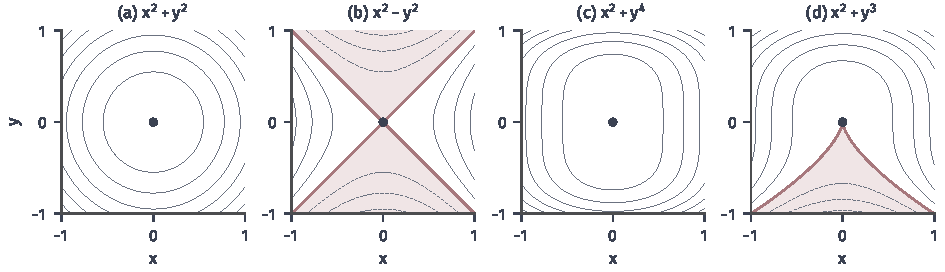
\includegraphics[width=160mm]{figures/03-optimization-evolution-and-signals/01-optimization/matplotlib/c1-stationary-types/figure.pdf}
  \caption{原点处四种驻点的等值线。灰线是等值线（虚线为负值），红色区域是函数值低于$f(\bm 0)=0$的点，红线是零等值线。(a) $x^2+y^2$：Hessian正定，严格最小点，附近没有更低的点。(b) $x^2-y^2$：Hessian不定，鞍点，红色区域从上下两侧伸到原点。(c) $x^2+y^4$：Hessian为$\operatorname{diag}(2,0)$，仍是严格最小点。(d) $x^2+y^3$：Hessian同为$\operatorname{diag}(2,0)$，但原点下方有更低的点，不是最小点。}
  \label{fig:opt-prob-stationary-types}
\end{figure*}

读者应从图中注意红色区域是否碰到原点：碰到就说明任意小的邻域里都有更低的点。(c)与(d)的二阶信息相同，红色区域却一有一无。

\paragraph{负曲率方向}
定理~\ref{thm:opt-prob-second-order}的必要性证明还包含一个可操作的信息。若驻点处存在方向$\bm d$使$\bm d^\top\nabla^2f(\bm x^\star)\bm d<0$，称$\bm d$为\term{负曲率方向}（negative curvature direction）。沿这个方向，一阶变化为零，函数却以$\frac{t^2}{2}\bm d^\top\bm H\bm d$的速度下降。图~\ref{fig:opt-prob-saddle-curvature}以$f(x,y)=x^2-y^2$为例：沿$(1,0)$方向函数向上弯，沿$(0,1)$方向向下弯，沿$(1,1)/\sqrt2$方向二阶项恰好为零。站在鞍点上，梯度不会指出任何下降方向，Hessian的负特征向量却指出了一条。第~\ref{chap:opt-smooth}章将利用这一判断讨论怎样离开鞍点。

\begin{figure*}[!htbp]
  \centering
  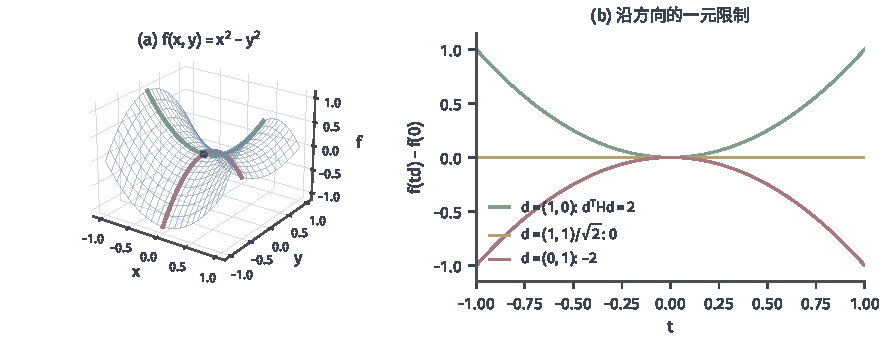
\includegraphics[width=150mm]{figures/03-optimization-evolution-and-signals/01-optimization/matplotlib/c1-saddle-curvature/figure.pdf}
  \caption{鞍点与负曲率方向。(a) 曲面$f(x,y)=x^2-y^2$，绿色曲线是沿$x$轴的截线（向上弯），红色曲线是沿$y$轴的截线（向下弯），黑点是驻点$\bm 0$。(b) 沿单位方向$\bm d$的一元限制$f(t\bm d)-f(\bm 0)=t^2\bm d^\top\bm H\bm d/2$，其中$\bm H=\operatorname{diag}(2,-2)$：方向$(1,0)$曲率为$2$，$(1,1)/\sqrt2$为$0$，$(0,1)$为$-2$，后者是负曲率方向。}
  \label{fig:opt-prob-saddle-curvature}
\end{figure*}

把本节与上一节合起来看：对一般光滑目标，梯度为零、Hessian正定只给出局部结论；对凸目标，梯度为零已经给出全局结论；对强凸目标，全局最优解还唯一，并且目标差控制到它的距离。条件越强，局部计算能推出的结论越强。
